\subsection{Second Experience}

\subsubsection{Python UDP Implementation (Loopback)}

After setting up a Python environment and running both scripts, we got the
following output:

\begin{figure}[htbp]
	\centering
	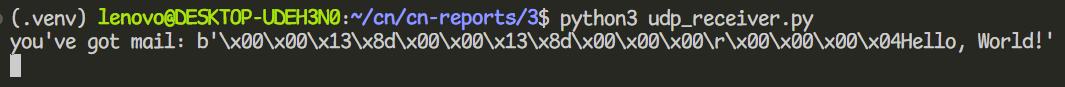
\includegraphics[width=1\linewidth]{img/second_exp/1.png}
	\caption{Receiver Output}\label{fig:2_1}
\end{figure}

\begin{figure}[htbp]
	\centering
	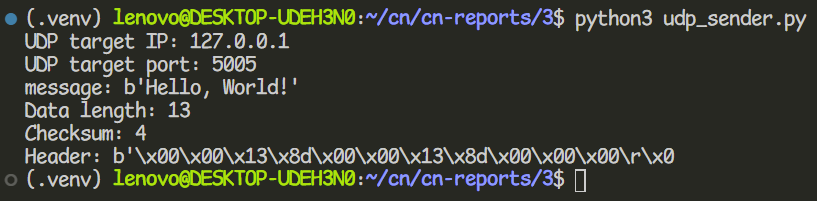
\includegraphics[width=1\linewidth]{img/second_exp/2.png}
	\caption{Sender Output}\label{fig:2_2}
\end{figure}

We can see that the received header matches the data sent by the sender, and
the IP is 127.0.0.1 as we were listening to that specific ip-port combination.

To further analyze the UDP package, we opened Wireshark and looked for the UDP package.

\subsubsection{Python UDP Implementation (P2P)}